\documentclass[12pt,a4paper]{article}

\usepackage[margin=1in]{geometry}
\usepackage{setspace}
\usepackage{graphicx}
\usepackage{amsmath}
\usepackage{hyperref}
\hypersetup{hidelinks}
\usepackage{pgfgantt}
\usepackage[nonumberlist,acronym,nomain]{glossaries}
\loadglsentries{acronyms.tex}

\usepackage{algorithm}
\usepackage{algpseudocode}



\usepackage{xcolor}
\usepackage{lmodern}
\usepackage[T1]{fontenc}
\usepackage{tikz}
\usepackage{subcaption}
\usetikzlibrary{positioning,arrows.meta}
%------------------------------------------------
% Custom colors
%------------------------------------------------
\definecolor{timelineblue}{RGB}{27,82,158}
\definecolor{timelinegreen}{RGB}{91,153,51}
\definecolor{timelinepurple}{RGB}{124,89,185}

\definecolor{phaseblue}{RGB}{232,241,252}
\definecolor{phasegreen}{RGB}{238,246,231}
\definecolor{phasepurple}{RGB}{243,237,250}

\definecolor{headerblue}{RGB}{8,35,78}
\definecolor{gridgray}{RGB}{205,205,205}
\usetikzlibrary{
    positioning,
    arrows.meta,
    fit,
    calc,
    shapes.geometric
}


\begin{document}

\begin{titlepage}
    \centering
    
    {\Large Aalen University of Applied Science \par}
    \vspace{0.5cm}
    {\large Faculty of Electronics and Computer Science \par}
      \vspace{1cm}
    {\Large PhD Research Proposal \par}
    \vspace{6cm}
    
    {\Huge \textbf{Application-Oriented MAC Scheduling and Resource Allocation for DECT-2020 NR Industrial IoT Networks} \par}
    
    \vspace{1.5cm}
    
    
    
    \vspace{6cm}
    
    \begin{flushleft}
    \textbf{Submitted by:} Ashuqullah Alizai \\
    \textbf{Email:} ashuqullah.alizai@hs-aalen.de\\
    \textbf{Supervisor:} Prof. Dr. Stephan Ludwig \\
    \textbf{Department:} Communications  \\
    \end{flushleft}
    
    \vfill
    
    {\large \today \par}
    
\end{titlepage}




\begin{abstract}

\gls{nr} is an \gls{etsi}-standardized wireless access technology designed to support \gls{iiot} and massive machine-type communication applications through flexible, decentralized, and private wireless deployments. Recent studies have demonstrated its potential for reliable and low-latency communication in industrial environments. However, existing research primarily focuses on protocol evaluation, performance characterization, and individual protocol enhancements, while comprehensive application-oriented \gls{mac} scheduling and resource-allocation approaches remain limited.

Industrial applications impose heterogeneous communication requirements. Deterministic control and sensor--actuator applications require predictable communication cycles with bounded latency and low jitter, reliability-critical applications require highly dependable packet delivery, and energy-constrained sensing applications require long device sleep durations while satisfying application-specific latency constraints. Supporting these requirements requires appropriate scheduling and resource allocation while accounting for practical protocol and hardware constraints.

This research investigates application-oriented \gls{mac} scheduling and resource allocation for \gls{nr} industrial networks. Rather than relying on a single generic scheduling configuration, the proposed approach develops configurable mechanisms for deterministic communication, reliability-oriented communication, and energy-efficient sensing. The research further investigates resource redundancy and multi-channel operation for reliability-oriented communication, as well as practical timing constraints associated with \gls{tdd} operation, \gls{rx}-to-\gls{tx} turnaround, processing delays, and schedule dissemination.

The proposed methodology combines \gls{mac}-layer design, implementation, controlled experimentation, and measurement-based validation on a real \gls{nr} hardware platform. The expected outcome is an experimentally validated, application-oriented \gls{mac} framework that maps industrial communication requirements to suitable scheduling and resource-allocation configurations while characterizing their trade-offs in terms of latency, jitter, reliability, resource utilization, scalability, and energy efficiency. The resulting findings are expected to provide practical design guidelines for future industrial DECT-2020 NR deployments.

\end{abstract}

\section{Introduction}

Industrial wireless communication systems are increasingly used to support monitoring, control, automation, and coordination tasks in modern production environments. Applications such as factory automation, closed-loop control, condition monitoring, mobile robotics, and battery-powered sensing impose substantially different requirements regarding latency, jitter, reliability, scalability, and energy consumption \cite{willigWirelessTechnologyIndustrial2005,vitturiIndustrialWirelessNetworks2013,wollschlaegerFutureIndustrialCommunication2017a}. Consequently, a single wireless technology or network configuration may not satisfy all industrial use cases. Heterogeneous communication architectures combining different local and cellular technologies have therefore emerged as an important enabler of Industry~4.0 and smart manufacturing \cite{alizaiHeterogeneousCommunicationNetworks2023a,karrenbauerFutureIndustrialNetworking2019a,aschenbrennerFlexiCell5GLocationbased2022a}.

\gls{nr} is an \gls{etsi}-standardized radio access technology developed within the IMT-2020 framework for local-area and massive-machine-type communication. The technology supports autonomous and decentralized network formation without requiring the conventional base-station and core-network architecture of cellular systems \cite{kovalchukovDECT2020NewRadio2022,perez-guiraoDECTNRUnveiling2022}. It is intended for applications such as industrial monitoring, building automation, smart metering, professional audio, critical-infrastructure communication, and other \gls{iot}/\gls{iiot} scenarios \cite{durreDECT2020NRProfessional2024,poetsProfessionalNetworkedAudio2025,biswasReliableLowLatencyCommunications2024}. Its operation is defined for dedicated DECT spectrum and additional frequency bands subject to the applicable regional regulatory framework \cite{etsi_tr103943}.

The DECT-2020 NR protocol architecture is defined in the ETSI TS~103~636 series. The \gls{phy} layer specifies radio transmission and reception procedures, while the \gls{mac} layer defines mechanisms for channel access, beaconing, association, random access, resource allocation, scheduled transmission, and group communication \cite{etsi_ts103636_1,etsi_ts103636_3,etsi_ts103636_4}. Radio devices may operate as \glspl{ft}, \glspl{pt}, or simultaneously in both roles, enabling point-to-point, point-to-multipoint, and multi-hop network topologies. Although the standard specifies the messages, timing relationships, and resource structures required for interoperable operation, the selection, configuration, and implementation of application-specific scheduling and resource-allocation policies remain implementation-dependent design tasks.

In this research, \textit{resource allocation} denotes the assignment of radio resources, including frequency channels, subslots, slots, and transmission opportunities, to communicating devices. \textit{\gls{mac} scheduling} denotes the policy used to determine how and when the allocated resources are used by individual devices or groups of devices. Random access provides contention-based opportunities for network entry and unscheduled communication, whereas group assignment enables devices with related communication requirements to be coordinated through common resource configurations. Together, these mechanisms determine how available radio resources are organized and used to satisfy application-specific communication requirements.

Existing studies have demonstrated that DECT-2020 NR can satisfy important IMT-2020 performance requirements and support low-latency and massive-device communication under selected configurations \cite{dhanwaniAssessmentCandidateTechnology2020,pennerURLLCPerformanceEvaluation2021,smidaETSIDECT2020Component2023}. Experimental investigations have further evaluated physical-layer performance, communication range, energy consumption, and suitability for industrial and professional-audio environments \cite{wassmannPerformanceDECT2020NR2024,haqueDECT2020NRLink2025,grafWhatExpectWhen2026,durreDECT2020NRProfessional2024}. However, much of the current literature concentrates on feasibility assessment, link- and system-level performance, or individual protocol enhancements rather than on an integrated application-oriented approach to \gls{mac} scheduling and resource allocation.

Industrial applications require different \gls{mac}-layer behavior according to their communication requirements. This research considers three representative communication classes: deterministic control communication requiring predictable communication cycles, bounded latency, and low jitter; reliability-oriented communication requiring highly dependable packet delivery; and energy-efficient sensing requiring reduced radio activity and long device sleep periods while satisfying application-specific latency constraints. These application classes can require different scheduling and resource-allocation configurations and introduce trade-offs among timing predictability, reliability, resource utilization, scalability, and energy consumption.

Practical implementation constraints must also be considered when designing such mechanisms. DECT-2020 NR communication performance is influenced not only by the resource structures and procedures defined by the standard but also by hardware and protocol timing effects, including \gls{tdd} operation, processing delays, schedule-dissemination overhead, radio-state transitions, and \gls{rx}-to-\gls{tx} turnaround time. Preliminary measurements on the available DECT-2020 NR hardware platform indicate that implementation-related delays can contribute substantially to end-to-end communication latency, particularly for short-packet and request--response communication. Consequently, application-oriented scheduling and resource-allocation configurations must be designed and evaluated with explicit consideration of practical platform constraints.

Accordingly, this research aims to design, implement, and experimentally validate application-oriented \gls{mac} scheduling and resource-allocation mechanisms for \gls{nr} industrial networks. The work focuses on deterministic communication, reliability-oriented communication, and energy-efficient sensing and investigates how scheduling, resource allocation, random access, group assignment, transmission redundancy, and multi-channel operation can be configured according to their respective application requirements. The overall objective is to establish an experimentally validated, application-oriented \gls{mac} framework that maps industrial communication requirements to suitable scheduling and resource-allocation configurations while characterizing the resulting trade-offs in latency, jitter, reliability, resource utilization, scalability, and energy efficiency.

\section{Background and Related Work}
\subsection{Industrial Wireless Communication Requirements}

Industrial automation and \gls{iiot} applications require wireless communication systems capable of supporting heterogeneous and, in some cases, conflicting communication requirements. As illustrated in Figure~\ref{fig:industrial_requirements}, modern industrial environments encompass a wide range of applications, including industrial control, monitoring and sensing, safety and protection, mobile and logistics systems, and multimedia or maintenance services. Although these applications may coexist within the same communication infrastructure, their requirements differ substantially in terms of latency, jitter, reliability, scalability, energy consumption, and \gls{qos} \cite{willigWirelessTechnologyIndustrial2005,vitturiIndustrialWirelessNetworks2013,wollschlaegerFutureIndustrialCommunication2017a,boyesIndustrialInternetThings2018,sisinniIndustrialInternetThings2018}.

\begin{figure}[htbp]
    \centering
    
\includegraphics[width=\textwidth]{figures/IndustrialApp.png}
    \caption{Representative industrial applications and their corresponding wireless communication requirements.}
    \label{fig:industrial_requirements}
\end{figure}

Industrial control applications, such as \glspl{plc}, robotic systems, and motion control, require predictable communication with bounded latency, low jitter, and high packet-delivery reliability. Monitoring and sensing applications generally tolerate less stringent timing constraints but place greater emphasis on low energy consumption, long device lifetime, and connectivity for large numbers of devices. Safety and protection applications, including alarms and emergency signaling, require timely and highly reliable message delivery. Mobile and logistics applications, such as autonomous guided vehicles (AGVs), tracking, and localization, additionally require robust communication under mobility and changing radio conditions. Other industrial services, including video, diagnostics, configuration, and software updates, may have less stringent timing requirements but introduce additional traffic and resource-management demands \cite{willigWirelessTechnologyIndustrial2005,vitturiIndustrialWirelessNetworks2013,wollschlaegerFutureIndustrialCommunication2017a,sisinniIndustrialInternetThings2018}.

These heterogeneous requirements create fundamental trade-offs in wireless resource management. Reserving communication resources can improve timing predictability and reliability but may reduce resource flexibility, while contention-based access can improve resource utilization for sporadic traffic at the cost of less predictable access delay. Similarly, extending device sleep intervals can reduce energy consumption but may increase response latency. Supporting heterogeneous industrial applications therefore requires communication mechanisms that can balance application-specific timing, reliability, resource-utilization, scalability, and energy requirements rather than relying on a single fixed communication configuration.

The diversity of industrial requirements has motivated heterogeneous communication infrastructures that combine different wired and wireless technologies according to application, coverage, and performance needs \cite{alizaiHeterogeneousCommunicationNetworks2023a,karrenbauerFutureIndustrialNetworking2019a,aschenbrennerFlexiCell5GLocationbased2022a}. While such architectures provide flexibility, they can also increase deployment complexity and network-management overhead. This has created interest in wireless technologies that support private and locally managed communication while providing configurable mechanisms for different traffic and application requirements.

DECT-2020 NR is relevant in this context because its decentralized architecture and flexible \gls{mac}-layer mechanisms support scheduled and contention-based communication, resource allocation, random access, and group-oriented operation \cite{etsi_ts103636_1,etsi_ts103636_4,perez-guiraoDECTNRUnveiling2022,kovalchukovDECT2020NewRadio2022}. However, the ability of a DECT-2020 NR deployment to satisfy heterogeneous industrial requirements depends not only on the capabilities provided by the standard but also on how these \gls{mac}-layer mechanisms are configured and coordinated for particular application requirements. This relationship motivates the application-oriented scheduling and resource-allocation problem investigated in this research.

\subsection{DECT-2020 NR Architecture and MAC Operation}
\label{subsec:dect-architecture-mac}

DECT-2020 NR supports autonomous and decentralized network formation for local wireless communication without requiring the permanently deployed base-station and core-network infrastructure characteristic of conventional cellular systems \cite{kovalchukovDECT2020NewRadio2022,dhanwaniAssessmentCandidateTechnology2020}. Its protocol architecture and radio procedures are specified in the ETSI TS~103~636 series \cite{etsi_ts103636_1,etsi_ts103636_2,etsi_ts103636_3,etsi_ts103636_4}. Figure~\ref{fig:dectnr_architecture_mac} summarizes the protocol architecture, device roles, communication paths, and principal MAC-layer operation considered in this research.

The protocol stack comprises the application layer, the \gls{mac} layer, the \gls{phy} layer, and the RF front-end. The application layer represents industrial services and their communication requirements. The \gls{phy} layer provides the radio-transmission functions, including modulation, coding, numerology, channel structure, and transmission and reception procedures. Above it, the \gls{mac} layer coordinates communication through mechanisms including beaconing, network discovery, association, random access, resource allocation, scheduled transmission, feedback, and group communication \cite{etsi_ts103636_2,etsi_ts103636_3,etsi_ts103636_4}.

A DECT-2020 NR device may operate as a \gls{ft}, a \gls{pt}, or in both roles. An \gls{ft} coordinates communication within a local network by transmitting beacons, managing radio resources, and distributing scheduling and control information. Associated \glspl{pt} use the available communication resources to exchange application data and provide acknowledgement, status, or other feedback information. Devices capable of operating in both roles can additionally support multi-hop communication, enabling more complex network structures \cite{etsi_ts103636_1,etsi_ts103636_4}. The present research primarily considers controlled star-topology deployments in which one \gls{ft} coordinates multiple \glspl{pt}. This topology provides a reproducible setting for investigating application-oriented scheduling and resource-allocation mechanisms.

As illustrated in the lower part of Figure~\ref{fig:dectnr_architecture_mac}, communication is organized around periodic beacon transmissions and associated MAC procedures. The \gls{ft} transmits beacon information that supports network identification, synchronization, control, and resource coordination. Nearby \glspl{pt} scan the available radio channels, detect suitable beacon transmissions, and identify networks with which they can communicate. A \gls{pt} may subsequently initiate association, during which the information required for participation in the network is established \cite{etsi_ts103636_4}.

Following association, communication resources must be assigned to the participating devices. Depending on the selected configuration and traffic characteristics, transmission opportunities may be provided through scheduled resource allocation or contention-based access. Scheduling information coordinates when and on which resources the \glspl{pt} may transmit or receive. During the communication phase, application and control data are exchanged using these resources, followed by acknowledgement, reception-status, or other feedback information. This information can subsequently be used when configuring resource assignments and scheduling decisions for later communication cycles.

The distinction between \textit{resource allocation} and \textit{scheduling} is important for the proposed research. Resource allocation determines which radio resources---for example, channels, slots, subslots, or transmission opportunities---are made available to devices, whereas scheduling determines how these resources are organized and assigned over time according to application and network requirements. Random access and group assignment provide additional mechanisms for coordinating unscheduled traffic and devices with related communication requirements. The interaction of these mechanisms determines the resulting timing predictability, reliability, resource utilization, scalability, and energy behavior of the network.

The DECT-2020 NR specifications define the available resource structures, signaling procedures, and communication mechanisms but do not prescribe a single application-specific scheduling policy \cite{etsi_ts103636_3,etsi_ts103636_4}. Consequently, implementations can configure and coordinate these mechanisms differently according to deployment requirements. This flexibility is particularly relevant for industrial applications because deterministic control, reliability-critical communication, and energy-constrained sensing impose different and potentially conflicting requirements. Determining how DECT-2020 NR MAC mechanisms should be configured for these application classes therefore constitutes the scheduling and resource-allocation problem addressed in this research.

\begin{figure}[htbp]
    \centering
    
\includegraphics[width=\textwidth]{figures/archetictur.png}
    \caption{DECT-2020 NR architecture and MAC operation. The upper part illustrates the protocol stack, device roles, and principal uplink and downlink communication paths. The lower part summarizes the principal MAC-layer communication procedure from beacon transmission and network discovery through association, resource scheduling, data transmission, feedback, and schedule update.}
    \label{fig:dectnr_architecture_mac}
\end{figure}
% =====================================================

\subsection{Scheduling and Resource Allocation in DECT-2020 NR Wireless Networks}
\label{subsec:scheduling}

Scheduling and resource allocation are fundamental \gls{mac}-layer functions that determine how multiple devices share limited wireless communication resources. Resource allocation determines which communication resources are assigned to individual devices or groups, whereas scheduling determines when and how these resources are used. In wireless systems, these decisions must account for factors such as varying channel conditions, interference, transmission errors, device availability, and half-duplex communication constraints \cite{luFairSchedulingWireless1999a,fattahOverviewSchedulingAlgorithms2002a}.

Traditional wireless scheduling algorithms have primarily been developed to improve aggregate throughput, spectral efficiency, fairness, or statistical \gls{qos}. Representative approaches include round-robin, proportional-fair, maximum-rate, earliest-deadline-first, and priority-based scheduling. Depending on their design objectives, these approaches balance packet delay, fairness, channel utilization, and changing radio conditions \cite{andrewsProvidingQualityService2001,fattahOverviewSchedulingAlgorithms2002a}. Although these principles provide useful foundations, industrial wireless communication introduces additional requirements related to timing predictability, reliability, and energy consumption.

For periodic industrial control traffic, scheduling must provide predictable transmission opportunities so that communication can be completed within the required application cycle while limiting latency variation and jitter. Reliability-oriented communication may require additional transmission opportunities, resource redundancy, or channel diversity to increase the probability of successful packet delivery. In contrast, battery-powered sensing applications benefit from sparse and predictable communication opportunities that allow devices to remain in low-power states for extended periods. Consequently, no single scheduling configuration is expected to be optimal for all industrial traffic classes.

In the controlled star-topology configuration considered in this research, the \gls{ft} coordinates communication resources for multiple associated \glspl{pt}. Following network discovery and association, communication resources can be assigned to the participating devices and the corresponding scheduling information distributed through the available control mechanisms. Resource assignment may involve the selection of frequency channels, slots, subslots, and transmission opportunities, while the resulting schedule determines when individual devices or groups are permitted to transmit or receive \cite{etsi_ts103636_3,etsi_ts103636_4}.

The scheduling problem is further constrained by the timing structure and practical operation of DECT-2020 NR. Resource assignments must respect the available radio-resource structure, \gls{tdd} operation, signaling overhead, processing time, and the timing required for transitions between transmission and reception. These constraints are particularly relevant for short communication cycles, where hardware and protocol timing can constitute a significant fraction of the overall communication delay. Scheduling mechanisms developed for other wireless systems therefore cannot be transferred directly without considering the specific resource structure and timing behavior of DECT-2020 NR.

The DECT-2020 NR specifications define the available resource structures, signaling procedures, and communication mechanisms but do not prescribe a universal application-specific scheduling policy \cite{etsi_ts103636_3,etsi_ts103636_4}. Implementers must therefore determine how resources are assigned among devices, how scheduled and contention-based transmission opportunities are configured, and how these configurations are selected according to deployment requirements. This implementation flexibility creates an important design space in which different scheduling and resource-allocation configurations may produce substantially different latency, jitter, reliability, scalability, and energy-consumption behavior.

Optimization, priority-aware, and delay-aware resource-allocation techniques developed for other wireless and cellular systems provide useful methodological foundations \cite{andrewsProvidingQualityService2001,liuEfficientResourceAllocation2024,bahetiPriorityawareRadioResource2026nr1}. However, these approaches generally assume different network architectures, frame structures, control procedures, and resource-management mechanisms. Their direct applicability to DECT-2020 NR is therefore limited. This motivates the investigation of application-oriented scheduling and resource allocation specifically for industrial DECT-2020 NR networks, where configurations are selected according to the requirements of deterministic control, reliability-oriented communication, and energy-efficient sensing.
% =====================================================

\subsection{Random Access and Group-Based Communication}
\label{subsec:random_access}

Random access is an essential mechanism in wireless networks that enables devices to transmit when dedicated communication resources have not yet been assigned or when sporadic data must be delivered outside an existing schedule. Its performance is strongly influenced by the number of contending devices, contention-window configuration, collision probability, retransmission strategy, and access-response timing. As network density increases, contention-based access may result in repeated collisions, increased access delay, reduced reliability, and higher energy consumption because devices repeatedly attempt channel access or remain active while waiting for network responses \cite{andrewsProvidingQualityService2001,fattahOverviewSchedulingAlgorithms2002a}.

Within DECT-2020 NR, random access supports several fundamental communication procedures, including initial network association and contention-based data transmission. The ETSI specification defines the signaling messages, timing relationships, and protocol procedures required for random access, while leaving the selection of operational parameters to the system implementation \cite{etsi_ts103636_4}. Consequently, network performance depends not only on the standardized protocol but also on how random-access opportunities are configured for a particular deployment. Recent work has demonstrated that random-access delay in DECT-2020 NR can be reduced by estimating the number of active devices and dynamically adapting the access procedure, illustrating the importance of deployment-aware parameter configuration \cite{gaidamakaOptimizingDelaysRandom2025}.

For industrial wireless applications, random access is particularly important for event-driven communication, including alarms, fault notifications, and sporadic sensor updates, where transmission requests occur unpredictably and cannot always be reserved in advance \cite{willigWirelessTechnologyIndustrial2005,vitturiIndustrialWirelessNetworks2013,wollschlaegerFutureIndustrialCommunication2017a}. Since these transmissions cannot be scheduled deterministically beforehand, reserving dedicated communication resources for every possible event would lead to inefficient resource utilization and reduced spectrum efficiency \cite{andrewsProvidingQualityService2001}. Conversely, relying exclusively on contention-based access under high network load may result in increased collision probability, longer access delays, and degraded reliability for time-critical applications \cite{fattahOverviewSchedulingAlgorithms2002a,gaidamakaOptimizingDelaysRandom2025}. Consequently, an industrial \gls{mac} design should combine deterministic scheduled resources for periodic traffic with carefully configured random-access opportunities for sporadic and event-driven communication, thereby balancing responsiveness, reliability, and resource efficiency.

Group-based communication provides an additional mechanism for improving scheduling efficiency in networks containing large numbers of devices with similar communication characteristics. Devices may be grouped according to application cycle, traffic periodicity, latency requirements, reliability constraints, or energy-consumption objectives. Rather than scheduling each device independently, the coordinator may allocate common communication resources or shared transmission opportunities to an entire group. Such coordination reduces scheduling overhead, simplifies schedule dissemination, and can improve resource utilization, particularly in industrial monitoring and control systems where many devices exhibit similar communication patterns \cite{etsi_ts103636_4}.

Despite its potential benefits, group-based communication introduces several scheduling challenges. Devices assigned to the same group must remain sufficiently synchronized to ensure coordinated resource usage, while heterogeneous communication requirements within a group may increase waiting time, reduce resource utilization, or compromise deterministic performance \cite{willigWirelessTechnologyIndustrial2005,vitturiIndustrialWirelessNetworks2013}. Consequently, effective group formation should consider application timing, traffic characteristics, device capabilities, latency requirements, and the availability of communication resources to achieve an appropriate balance between efficiency and quality of service \cite{andrewsProvidingQualityService2001,fattahOverviewSchedulingAlgorithms2002a}. These trade-offs become increasingly significant as the number of connected devices grows and multiple heterogeneous industrial applications coexist within the same wireless network \cite{wollschlaegerFutureIndustrialCommunication2017a}.

Although DECT-2020 NR provides standardized signaling procedures and
resource-allocation mechanisms that support both contention-based access and
group-oriented communication \cite{etsi_ts103636_4}, our systematic review of
the current DECT-2020 NR literature indicates that existing studies have
primarily concentrated on protocol architecture, implementation, performance
evaluation, and isolated optimization problems, while application-oriented
\gls{mac} scheduling and resource allocation for heterogeneous industrial
applications have received comparatively limited attention
\cite{gaidamakaOptimizingDelaysRandom2025,kovalchukovDECT2020NewRadio2022}.
In particular, few studies jointly consider application requirements,
random-access configuration, device grouping, schedule dissemination, and
practical hardware timing within a unified scheduling and resource-allocation
framework. Addressing these challenges forms one of the central objectives of
the proposed research.

% =======================================================================================================================================================

\subsection{Research Gap}
\label{subsec:research_gap}

The existing DECT-2020 NR literature has established the feasibility of the technology, evaluated its performance under selected configurations, and proposed enhancements to individual protocol mechanisms
\cite{dhanwaniAssessmentCandidateTechnology2020,
anttonenEnablingMassiveMachine2021a,
pennerURLLCPerformanceEvaluation2021,
wassmannPerformanceDECT2020NR2024,
ahmadMACProtocolReducing2024,
nihtilaEnergyConsumptionDECT20202022}.
However, the available studies do not yet provide a comprehensive and experimentally validated methodology for configuring \gls{mac} scheduling and resource allocation according to heterogeneous industrial application requirements. Based on the preceding review, five closely related research gaps are identified.

\textbf{1) Deterministic communication:}
Periodic control and sensor--actuator applications require predictable communication cycles, bounded latency, and low jitter. Existing DECT-2020 NR studies have primarily characterized latency, reliability, and packet-delivery performance under predefined system configurations
\cite{pennerURLLCPerformanceEvaluation2021,
smidaETSIDECT2020Component2023,
llagunoPhysicalLayerPerformance2024,
bandaraExperimentalValidationAnalysis2025}.
Limited guidance is available on how radio resources should be organized when application periods and communication deadlines do not align directly with the DECT-2020 NR timing structure. In particular, the relationship among application-cycle requirements, resource reservation, schedule repetition, schedule dissemination, and practical timing constraints requires further investigation to achieve predictable cycle-to-cycle communication behavior.

\textbf{2) Reliability-oriented resource allocation:}
Existing work has investigated outage reduction, multi-hop reliability, and resource-prioritization mechanisms
\cite{ahmadMACProtocolReducing2024,
ahmadMACLayerProtocolUltraReliable2025,
binasifIRSAssistedDECT2020NR2025}.
However, the coordinated configuration of redundant transmission opportunities and multiple DECT-2020 NR channels for reliability-critical communication in controlled industrial star networks remains insufficiently studied. The trade-offs among transmission redundancy, channel diversity, packet-delivery reliability, communication latency, and resource overhead therefore require systematic experimental characterization.

\textbf{3) Energy-efficient communication scheduling:}
Previous studies have characterized DECT-2020 NR device energy consumption and investigated energy-saving operation for routing devices
\cite{nihtilaEnergyConsumptionDECT20202022,
nihtilaEnergySavingRouter2022}.
Nevertheless, the relationship between application latency requirements and the scheduling of transmission, reception, and sleep intervals for battery-powered end devices remains insufficiently addressed. A key open question is how communication opportunities and receive windows can be configured to reduce radio activity while ensuring that application-specific communication deadlines are satisfied.

\textbf{4) Hardware-aware MAC design:}
A substantial part of the existing literature relies on analytical models, simulations, or predefined timing assumptions
\cite{dhanwaniAssessmentCandidateTechnology2020,
anttonenEnablingMassiveMachine2021a,
pennerURLLCPerformanceEvaluation2021}.
Real implementations introduce additional timing effects associated with processing, \gls{tdd} operation, radio-state transitions, schedule dissemination, and \gls{rx}-to-\gls{tx} turnaround
\cite{wassmannPerformanceDECT2020NR2024,
haqueDECT2020NRLink2025,
grafWhatExpectWhen2026}.
The extent to which these implementation constraints affect achievable scheduling behavior, particularly latency and jitter, remains insufficiently integrated into MAC-level design. Experimental characterization must therefore form part of the design process rather than serving only as post-implementation validation.

\textbf{5) Integrated application-oriented MAC configuration:}
The preceding gaps are closely interconnected. Deterministic control, reliability-critical communication, event-driven traffic, and energy-constrained sensing impose different and sometimes conflicting requirements on the same radio resources. Existing studies generally investigate individual performance dimensions or protocol mechanisms separately. A systematic approach for mapping application requirements to appropriate combinations of scheduled resources, random-access opportunities, group assignments, redundancy, multi-channel operation, and transmission/reception timing remains lacking.

Accordingly, the central research gap addressed by this proposal is the absence of an implemented and experimentally validated application-oriented \gls{mac} framework that systematically relates heterogeneous industrial communication requirements to suitable DECT-2020 NR scheduling and resource-allocation configurations. Addressing this gap requires the joint consideration of deterministic timing, communication reliability, energy-efficient operation, and practical hardware constraints rather than optimizing these aspects independently.

% =====================================================

\subsection{Research Objectives}
\label{subsec:research_objectives}

The main objective of this research is to design, implement, and experimentally
validate an application-oriented \gls{mac} framework for \gls{nr} industrial
networks that maps heterogeneous application requirements to suitable scheduling
and resource-allocation configurations.

To achieve this goal, the following specific objectives are defined:

\begin{itemize}

\item \textbf{Application requirements and MAC configuration:}
To derive and formalize the communication requirements of representative
industrial application classes, including deterministic control communication,
reliability-critical communication, and energy-efficient sensing, and to
identify the corresponding \gls{mac}-layer configuration parameters and
resource requirements.

\item \textbf{Deterministic communication:}
To design scheduling and resource-allocation mechanisms for periodic industrial
communication that provide predictable transmission opportunities, bounded
communication latency, and low cycle-to-cycle latency variation and jitter.

\item \textbf{Reliability-oriented communication:}
To develop and investigate resource-allocation mechanisms based on reserved
resources, transmission redundancy, channel diversity, and coordinated
multi-channel operation, and to characterize the resulting trade-offs among
packet-delivery reliability, latency, and resource overhead.

\item \textbf{Energy-efficient communication:}
To design transmission, reception, and sleep scheduling mechanisms for
battery-powered devices that reduce radio activity and extend sleep duration
while satisfying application-specific communication deadlines and
data-delivery requirements.

\item \textbf{Hardware-aware integration and experimental validation:}
To integrate the proposed mechanisms into a configurable \gls{mac} framework
and implement them on a real \gls{nr} hardware platform. The framework will
explicitly account for practical protocol and hardware timing constraints and
will be experimentally evaluated under representative industrial scenarios in
terms of latency, jitter, packet-delivery reliability, resource utilization,
scalability, and energy-related behavior.

\end{itemize}

The expected outcome is an experimentally validated, application-oriented
\gls{mac} framework that systematically relates industrial communication
requirements to appropriate DECT-2020 NR scheduling and resource-allocation
configurations while exposing the trade-offs among deterministic timing,
communication reliability, resource utilization, scalability, and
energy-efficient operation.

\section{Methodology}
\label{sec:methodology}

This research follows an iterative design--implement--evaluate methodology for
developing and experimentally validating application-oriented \gls{mac}
scheduling and resource-allocation mechanisms for \gls{nr}. Industrial
application requirements are first translated into measurable communication
constraints and corresponding \gls{mac}-layer design parameters. Candidate
mechanisms are then implemented on a real DECT-2020 NR platform and evaluated
through controlled experiments. The resulting measurements are used to
characterize performance trade-offs, identify implementation limitations, and
iteratively refine the proposed mechanisms.
The research is organized into five interconnected phases:

\begin{enumerate}

\item \textbf{Requirements analysis:}
translate representative industrial application requirements into measurable
communication constraints and \gls{mac}-layer design parameters;

\item \textbf{MAC configuration and scheduling design:}
develop application-oriented scheduling policies and resource-allocation
configurations using the mechanisms provided by the DECT-2020 NR standard
for deterministic, reliability-oriented, and energy-efficient communication;

\item \textbf{Hardware implementation:}
implement and integrate the proposed mechanisms on the available DECT-2020 NR
experimental platform;

\item \textbf{Experimental evaluation:}
evaluate the implemented mechanisms through controlled and repeatable
experiments under representative communication scenarios; and

\item \textbf{Validation and refinement:}
compare the proposed configurations with baseline operation, analyze the
resulting trade-offs, refine the mechanisms, and derive practical design
guidelines.

\end{enumerate}

Although presented sequentially, these phases form an iterative research
process. Observations obtained during implementation and experimentation are
fed back into the design phase so that practical protocol and hardware
constraints can be incorporated into subsequent refinements.

% =====================================================

\subsection{Application Requirements Analysis}
\label{subsec:requirements_analysis}

The first phase translates the three application classes identified in
Section~\ref{subsec:research_gap} into quantitative communication requirements
and corresponding \gls{mac}-layer design parameters. Rather than repeating the
application characteristics themselves, this phase establishes measurable
constraints that can be used to design and evaluate the proposed mechanisms.

For deterministic communication, relevant parameters include the application
period, communication deadline, permitted latency variation, and required
transmission periodicity. These parameters are used to determine suitable
resource-reservation intervals, scheduling periodicity, and transmission
opportunities.

For reliability-oriented communication, the requirements are expressed in
terms of target packet-delivery reliability, allowable communication latency,
and acceptable resource overhead. These requirements determine the
configurations to be investigated for transmission redundancy, resource
duplication, and multi-channel operation.

For energy-efficient sensing, the relevant parameters include reporting
intervals, maximum tolerable communication latency, reception requirements,
and allowable device activity. These constraints are used to determine
transmission opportunities, receive-window configurations, and feasible sleep
intervals.

The resulting requirement sets provide the input to the subsequent
\gls{mac}-mechanism design and define the criteria against which the
experimental results are evaluated.

% =====================================================

\subsection{Design of Application-Oriented MAC Mechanisms}
\label{subsec:mac_design}

Based on the derived requirements, configurable scheduling and
resource-allocation mechanisms are developed and investigated for each
application class.

For deterministic communication, the design investigates how periodic
application traffic can be mapped to the DECT-2020 NR resource and timing
structure. Candidate configurations vary resource-reservation intervals,
transmission opportunities, schedule repetition, and, where applicable,
group-based resource assignments. The objective is to determine configurations
that provide predictable communication opportunities while reducing
cycle-to-cycle latency variation and jitter.

For reliability-oriented communication, the design investigates different
degrees and placements of redundant transmission opportunities together with
channel diversity and coordinated multi-channel resource allocation. The
number of redundant resources, their temporal placement, and their distribution
across available channels are varied experimentally to characterize the
trade-off between packet-delivery reliability, communication latency, and
resource overhead.

For energy-efficient sensing, transmission and reception opportunities are
configured according to the reporting interval and maximum tolerable
application latency. Different receive-window intervals and device activity
patterns are investigated to determine how long devices can remain inactive
while still satisfying their communication requirements.

Random access and group assignment are treated as supporting configuration
mechanisms. Random-access opportunities are considered for asynchronous and
event-driven traffic, whereas group-based resource configurations are
investigated for devices with compatible communication requirements. Their
interaction with scheduled communication is evaluated where relevant to the
corresponding application scenario.

% =====================================================

\subsection{Implementation on the DECT-2020 NR Platform}
\label{subsec:hardware_implementation}

The proposed mechanisms are implemented and evaluated on a real DECT-2020 NR
hardware platform based on Nordic Semiconductor development boards supporting
the DECT-2020 NR protocol stack. The experimental network primarily follows a
controlled star topology consisting of one \gls{ft} coordinating multiple
\glspl{pt}, representing industrial sensor, actuator, and monitoring devices.

Implementation includes the configuration and modification of the available
\gls{mac}-layer parameters and communication procedures required to realize
the investigated scheduling and resource-allocation configurations. Internal
protocol information and externally observable communication events are
recorded where available to relate configured schedules to actual radio
behavior.

Because transmission and reception share the available radio hardware,
practical timing constraints must be considered during implementation. These
include \gls{tdd} operation, \gls{rx}-to-\gls{tx} turnaround time, processing
delay, radio-state transitions, schedule-dissemination overhead, and firmware
execution behavior. These effects are measured where possible and incorporated
into the interpretation and refinement of the proposed mechanisms.

% =====================================================

\subsection{Experimental Evaluation}
\label{subsec:experimental_evaluation}

The implemented mechanisms are evaluated through controlled experiments
corresponding to the three application classes. Within each experiment,
relevant configuration parameters are varied systematically while other
experimental conditions are kept constant where possible, enabling comparison
between candidate configurations and baseline operation.

Deterministic communication experiments use periodic traffic with defined
application cycles and communication deadlines. Resource-reservation and
scheduling configurations are varied to evaluate their effect on end-to-end
latency, latency variation, jitter, and the ability to satisfy the required
communication cycle.

Reliability-oriented experiments evaluate alternative redundancy and
multi-channel configurations under controlled communication conditions.
Transmission outcomes are recorded to determine how additional transmission
opportunities and channel diversity affect packet-delivery reliability,
latency, and resource consumption.

Energy-efficient experiments vary reporting intervals, transmission
opportunities, and receive-window configurations. Device active, receive, and
inactive periods are characterized to evaluate the trade-off between
communication responsiveness and energy-related behavior.

Where relevant, additional experiments investigate increasing numbers of
\glspl{pt} and heterogeneous traffic combinations to assess scalability and
the interaction between different communication requirements. Experimental
configurations are repeated to assess repeatability and to support statistical
characterization of the observed behavior.

% =====================================================

\subsection{Performance Evaluation Metrics}
\label{subsec:performance_metrics}

Evaluation metrics are selected according to the requirements of each
application class rather than assuming that a single performance metric is
sufficient for all scenarios. The principal metrics considered in this
research are:

\begin{itemize}

\item end-to-end communication latency and latency percentiles;

\item communication jitter and cycle-to-cycle latency variation;

\item packet-delivery ratio and packet-delivery reliability;

\item resource utilization and additional resource or signaling overhead;

\item device active, receive, transmit, and sleep durations, together with
      energy consumption or an appropriate energy-related estimate where
      measurable; and

\item scalability with increasing numbers of devices and communication demands.

\end{itemize}

Where appropriate, \glspl{cdf}, percentile-based measures, dispersion metrics,
and repeated-run statistics are used to characterize the distribution and
variability of the measured performance. Particular attention is given to
tail behavior and deadline violations in scenarios where predictable
communication is more important than average performance.

% =====================================================

\subsection{Validation, Comparative Analysis, and Design Refinement}
\label{subsec:validation}

The final methodological phase compares the proposed configurations with
appropriate baseline DECT-2020 NR operation under equivalent experimental
conditions. The purpose of the comparison is not to identify a single
universally optimal scheduler, but to determine which configurations are
suitable for particular industrial communication requirements and to quantify
the associated trade-offs.

For deterministic communication, the analysis focuses on timing
predictability, latency variation, jitter, and deadline satisfaction. For
reliability-oriented communication, the relationship among packet-delivery
reliability, redundancy, latency, and resource overhead is examined. For
energy-efficient sensing, the analysis focuses on the relationship among
device activity, sleep duration, communication latency, and application
requirements. Scalability is evaluated where relevant by increasing the
number of participating devices or communication demands.

Experimental observations are fed back into the mechanism-design phase to
refine configurations and account for practical implementation constraints.
The resulting analysis is used to derive application-oriented design
guidelines that relate industrial communication requirements to suitable
DECT-2020 NR scheduling and resource-allocation configurations.

% =====================================================
%======================================================

\subsection{Timeline}
\label{subsec:timeline}

The proposed doctoral research is planned over a period of three years and
follows an iterative process of requirements analysis, scheduling and
configuration design, hardware implementation, experimental evaluation, and
refinement, as illustrated in Figure~\ref{fig:research-timeline}. Although the
activities are organized into three main phases, implementation and experimental
findings are continuously fed back into the design process.

During the first year, the research focuses on a systematic review of the
DECT-2020 NR literature, analysis and formalization of industrial communication
requirements, development of the system model, and establishment and
characterization of the experimental platform. Initial investigations examine
how application requirements can be mapped to the scheduling,
resource-allocation, random-access, and group-related mechanisms provided by
DECT-2020 NR. The literature review and initial experimental characterization
provide the foundation for the subsequent research activities and associated
publications.

During the second year, the research concentrates on the design,
implementation, and experimental investigation of application-oriented
scheduling policies and resource-allocation configurations. For deterministic
communication, periodic resource reservation, schedule repetition, and
group-based scheduling configurations are investigated. For
reliability-oriented communication, the work examines transmission redundancy,
resource duplication, channel diversity, and coordinated multi-channel
operation. For energy-efficient sensing, transmission opportunities,
receive-window configurations, and sleep intervals are investigated according
to application-specific latency requirements. The selected configurations are
implemented on the DECT-2020 NR hardware platform and evaluated through
controlled experiments. Results obtained during this phase are progressively
prepared for conference and journal publication.

During the third year, the individual approaches are integrated and subjected
to comprehensive experimental evaluation and validation under representative
industrial communication scenarios. The analysis focuses on the trade-offs
among latency, jitter, packet-delivery reliability, resource utilization,
scalability, and energy-related behavior. Experimental findings are used to
refine the application-to-MAC configuration framework and derive practical
design guidelines for industrial DECT-2020 NR deployments. The final research
results are disseminated through peer-reviewed publications, followed by
completion and submission of the doctoral dissertation and preparation for the
doctoral defense.

\begin{figure}[htbp]
\centering

\resizebox{\textwidth}{!}{%
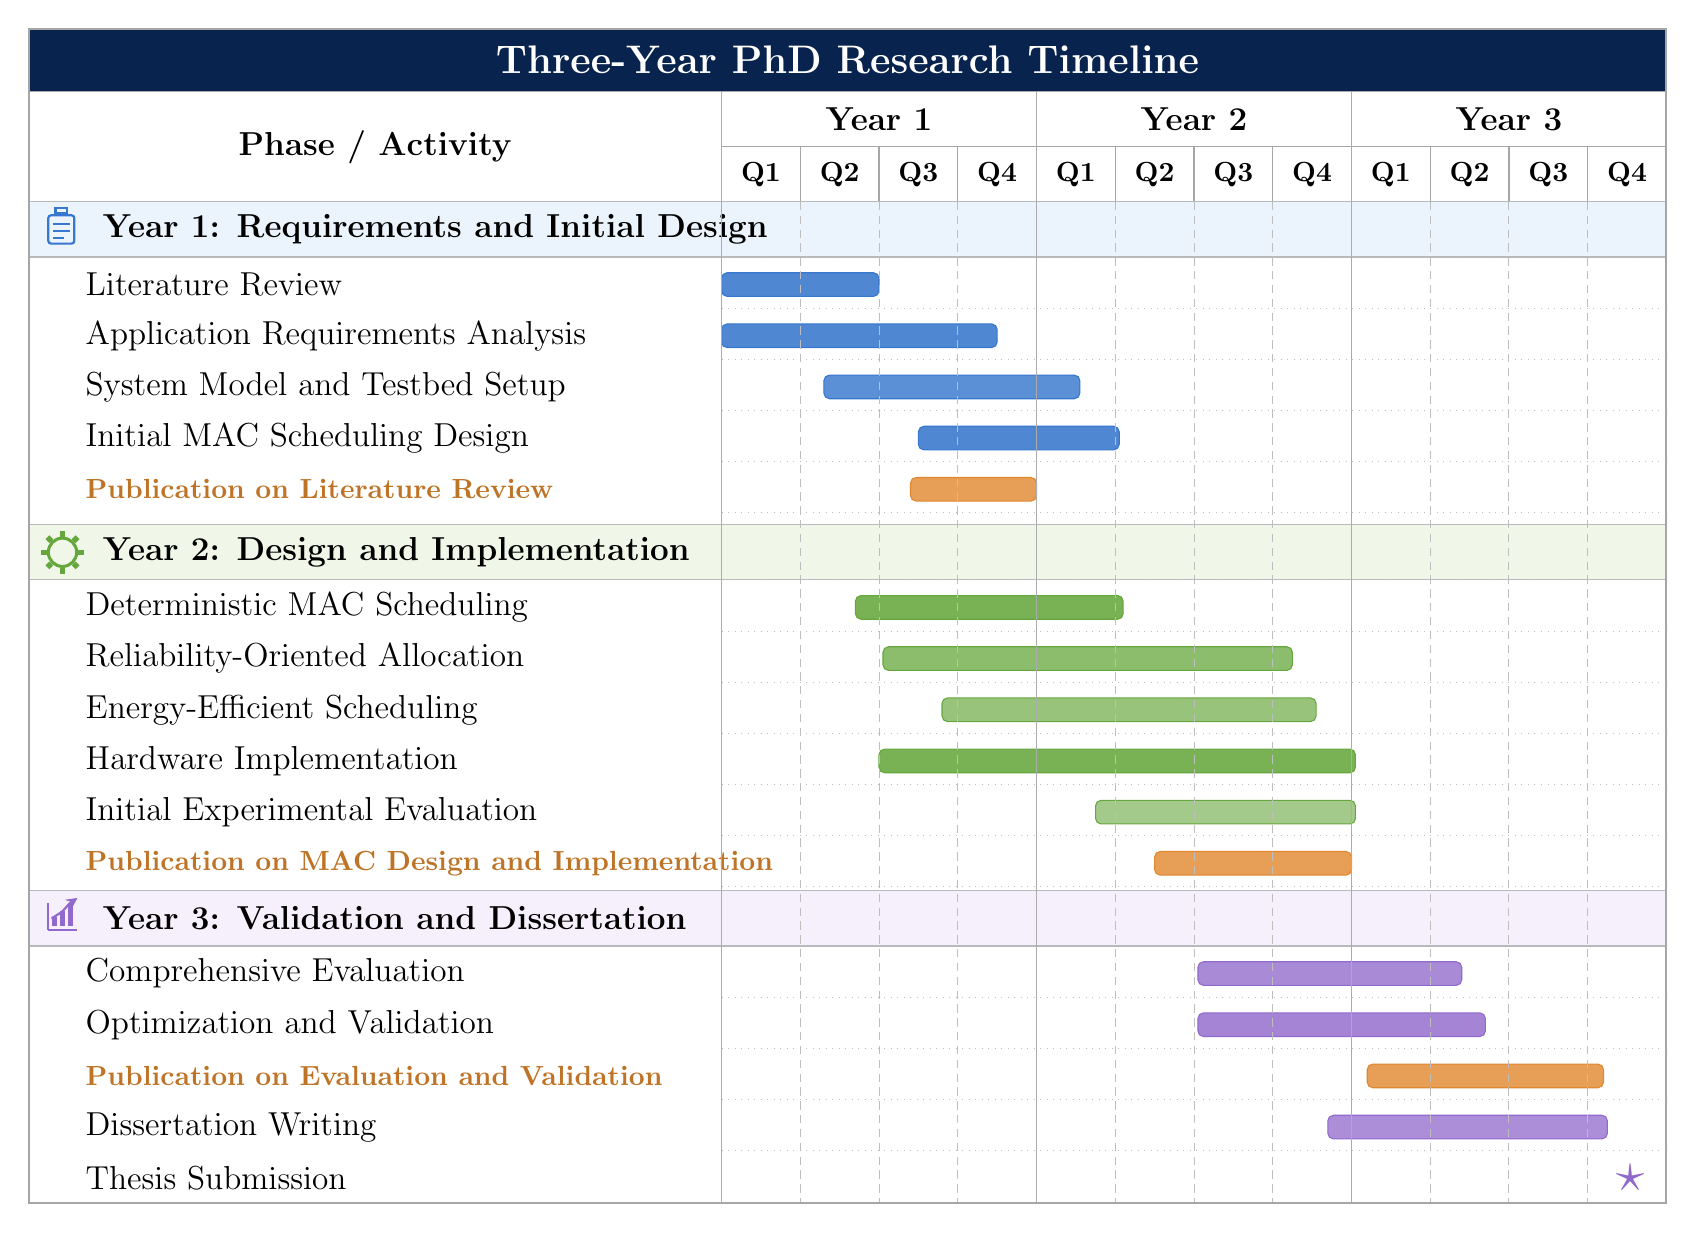
\begin{tikzpicture}[
    x=1cm,
    y=1cm,
    font=\small,
    task/.style={
        rounded corners=2pt,
        minimum height=0.28cm,
        inner sep=0pt
    }
]

% -------------------------------------------------
% Dimensions
% -------------------------------------------------
\def\labelwidth{8.8}
\def\quarterwidth{1.0}
\def\chartwidth{20.8}

% -------------------------------------------------
% Colors
% -------------------------------------------------
\definecolor{headerblue}{RGB}{8,35,78}
\definecolor{timelineblue}{RGB}{55,119,205}
\definecolor{timelinegreen}{RGB}{102,167,61}
\definecolor{timelinepurple}{RGB}{145,105,204}
\definecolor{timelineorange}{RGB}{225,135,45}

\definecolor{phaseblue}{RGB}{235,243,252}
\definecolor{phasegreen}{RGB}{240,247,233}
\definecolor{phasepurple}{RGB}{246,240,252}

\definecolor{gridgray}{RGB}{190,190,190}

% =================================================
% MAIN TITLE
% =================================================
\fill[headerblue] (0,0) rectangle (\chartwidth,-0.8);
\draw[gray!70] (0,0) rectangle (\chartwidth,-0.8);

\node[
    text=white,
    font=\bfseries\Large
] at (\chartwidth/2,-0.4)
{Three-Year PhD Research Timeline};

% =================================================
% LEFT HEADER: PHASE / ACTIVITY
% =================================================
\fill[white] (0,-0.8) rectangle (\labelwidth,-2.2);
\draw[gray!70] (0,-0.8) rectangle (\labelwidth,-2.2);

\node[
    font=\bfseries\large
] at (\labelwidth/2,-1.5)
{Phase / Activity};

% =================================================
% YEAR HEADERS
% =================================================
\foreach \x/\year in {
    8.8/Year 1,
    12.8/Year 2,
    16.8/Year 3
}{
    \fill[white] (\x,-0.8) rectangle ++(4,-0.7);
    \draw[gray!70] (\x,-0.8) rectangle ++(4,-0.7);

    \node[
        font=\bfseries\large
    ] at (\x+2,-1.15)
    {\year};
}

% =================================================
% QUARTER HEADERS
% =================================================
\foreach \i/\quarter in {
    0/Q1,1/Q2,2/Q3,3/Q4,
    4/Q1,5/Q2,6/Q3,7/Q4,
    8/Q1,9/Q2,10/Q3,11/Q4
}{
    \pgfmathsetmacro{\qx}{\labelwidth+\i}

    \fill[white]
        (\qx,-1.5)
        rectangle
        ++(\quarterwidth,-0.7);

    \draw[gray!70]
        (\qx,-1.5)
        rectangle
        ++(\quarterwidth,-0.7);

    \node[
        font=\bfseries
    ] at (\qx+0.5,-1.85)
    {\quarter};
}

% =================================================
% PHASE 1 HEADER
% =================================================
\fill[phaseblue] (0,-2.2) rectangle (\chartwidth,-2.9);
\draw[gray!55] (0,-2.2) rectangle (\chartwidth,-2.9);

% Small clipboard-style icon
\draw[timelineblue, line width=0.8pt, rounded corners=1pt]
    (0.25,-2.73) rectangle (0.58,-2.37);
\draw[timelineblue, line width=0.8pt]
    (0.34,-2.34) rectangle (0.49,-2.28);
\draw[timelineblue, line width=0.6pt]
    (0.31,-2.48) -- (0.52,-2.48);
\draw[timelineblue, line width=0.6pt]
    (0.31,-2.57) -- (0.52,-2.57);
\draw[timelineblue, line width=0.6pt]
    (0.31,-2.66) -- (0.45,-2.66);

\node[
    anchor=west,
    font=\bfseries\large
] at (0.82,-2.55)
{Year 1: Requirements and Initial Design};

% =================================================
% YEAR 1 ACTIVITIES
% =================================================
\node[anchor=west, font=\large]
    at (0.60,-3.25)
    {Literature Review};

\node[anchor=west, font=\large]
    at (0.60,-3.90)
    {Application Requirements Analysis};

\node[anchor=west, font=\large]
    at (0.60,-4.55)
    {System Model and Testbed Setup};

\node[anchor=west, font=\large]
    at (0.60,-5.20)
    {Initial MAC Scheduling Design};

\node[
    anchor=west,
    font=\normalsize\bfseries,
    text=timelineorange!85!black
] at (0.60,-5.85)
{Publication on Literature Review};

% Year 1 bars
\filldraw[
    task,
    fill=timelineblue!88,
    draw=timelineblue
]
(\labelwidth,-3.40)
rectangle
(\labelwidth+2.0,-3.10);

\filldraw[
    task,
    fill=timelineblue!88,
    draw=timelineblue
]
(\labelwidth,-4.05)
rectangle
(\labelwidth+3.50,-3.75);

\filldraw[
    task,
    fill=timelineblue!82,
    draw=timelineblue
]
(\labelwidth+1.30,-4.70)
rectangle
(\labelwidth+4.55,-4.40);

\filldraw[
    task,
    fill=timelineblue!88,
    draw=timelineblue
]
(\labelwidth+2.50,-5.35)
rectangle
(\labelwidth+5.05,-5.05);

% Year 1 publication bar
\filldraw[
    task,
    fill=timelineorange!80,
    draw=timelineorange
]
(\labelwidth+2.40,-6.00)
rectangle
(\labelwidth+4.00,-5.70);

% =================================================
% PHASE 2 HEADER
% =================================================
\fill[phasegreen] (0,-6.30) rectangle (\chartwidth,-7.00);
\draw[gray!55] (0,-6.30) rectangle (\chartwidth,-7.00);

% Small gear-style icon
\draw[
    timelinegreen,
    line width=1.1pt
]
(0.43,-6.65) circle (0.18);

\foreach \angle in {0,45,...,315}{
    \draw[
        timelinegreen,
        line width=2pt
    ]
    ($(0.43,-6.65)+(\angle:0.20)$)
    --
    ($(0.43,-6.65)+(\angle:0.27)$);
}

\node[
    anchor=west,
    font=\bfseries\large
] at (0.82,-6.65)
{Year 2: Design and Implementation};

% =================================================
% YEAR 2 ACTIVITIES
% =================================================
\node[anchor=west, font=\large]
    at (0.60,-7.35)
    {Deterministic MAC Scheduling};

\node[anchor=west, font=\large]
    at (0.60,-8.00)
    {Reliability-Oriented Allocation};

\node[anchor=west, font=\large]
    at (0.60,-8.65)
    {Energy-Efficient Scheduling};

\node[anchor=west, font=\large]
    at (0.60,-9.30)
    {Hardware Implementation};

\node[anchor=west, font=\large]
    at (0.60,-9.95)
    {Initial Experimental Evaluation};

\node[
    anchor=west,
    font=\normalsize\bfseries,
    text=timelineorange!85!black
] at (0.60,-10.60)
{Publication on MAC Design and Implementation};

% Year 2 bars
\filldraw[
    task,
    fill=timelinegreen!88,
    draw=timelinegreen
]
(\labelwidth+1.70,-7.50)
rectangle
(\labelwidth+5.10,-7.20);

\filldraw[
    task,
    fill=timelinegreen!75,
    draw=timelinegreen
]
(\labelwidth+2.05,-8.15)
rectangle
(\labelwidth+7.25,-7.85);

\filldraw[
    task,
    fill=timelinegreen!68,
    draw=timelinegreen
]
(\labelwidth+2.80,-8.80)
rectangle
(\labelwidth+7.55,-8.50);

\filldraw[
    task,
    fill=timelinegreen!88,
    draw=timelinegreen
]
(\labelwidth+2.00,-9.45)
rectangle
(\labelwidth+8.05,-9.15);

\filldraw[
    task,
    fill=timelinegreen!60,
    draw=timelinegreen
]
(\labelwidth+4.75,-10.10)
rectangle
(\labelwidth+8.05,-9.80);

% Year 2 publication bar
\filldraw[
    task,
    fill=timelineorange!80,
    draw=timelineorange
]
(\labelwidth+5.50,-10.75)
rectangle
(\labelwidth+8.00,-10.45);

% =================================================
% PHASE 3 HEADER
% =================================================
\fill[phasepurple] (0,-10.95) rectangle (\chartwidth,-11.65);
\draw[gray!55] (0,-10.95) rectangle (\chartwidth,-11.65);

% Small chart icon
\draw[
    timelinepurple,
    line width=0.8pt
]
(0.25,-11.45) -- (0.25,-11.10);

\draw[
    timelinepurple,
    line width=0.8pt
]
(0.25,-11.45) -- (0.62,-11.45);

\fill[timelinepurple]
    (0.30,-11.40) rectangle (0.36,-11.28);

\fill[timelinepurple]
    (0.40,-11.40) rectangle (0.46,-11.20);

\fill[timelinepurple]
    (0.50,-11.40) rectangle (0.56,-11.10);

\draw[
    timelinepurple,
    line width=0.8pt,
    -stealth
]
(0.29,-11.30)
--
(0.42,-11.22)
--
(0.52,-11.11)
--
(0.62,-11.04);

\node[
    anchor=west,
    font=\bfseries\large
] at (0.82,-11.30)
{Year 3: Validation and Dissertation};

% =================================================
% YEAR 3 ACTIVITIES
% =================================================
\node[anchor=west, font=\large]
    at (0.60,-12.00)
    {Comprehensive Evaluation};

\node[anchor=west, font=\large]
    at (0.60,-12.65)
    {Optimization and Validation};

\node[
    anchor=west,
    font=\normalsize\bfseries,
    text=timelineorange!85!black
] at (0.60,-13.30)
{Publication on Evaluation and Validation};

\node[anchor=west, font=\large]
    at (0.60,-13.95)
    {Dissertation Writing};

\node[anchor=west, font=\large]
    at (0.60,-14.60)
    {Thesis Submission};

% Year 3 bars
\filldraw[
    task,
    fill=timelinepurple!78,
    draw=timelinepurple
]
(\labelwidth+6.05,-12.15)
rectangle
(\labelwidth+9.40,-11.85);

\filldraw[
    task,
    fill=timelinepurple!82,
    draw=timelinepurple
]
(\labelwidth+6.05,-12.80)
rectangle
(\labelwidth+9.70,-12.50);

% Year 3 publication bar
\filldraw[
    task,
    fill=timelineorange!80,
    draw=timelineorange
]
(\labelwidth+8.20,-13.45)
rectangle
(\labelwidth+11.20,-13.15);

\filldraw[
    task,
    fill=timelinepurple!76,
    draw=timelinepurple
]
(\labelwidth+7.70,-14.10)
rectangle
(\labelwidth+11.25,-13.80);

% Thesis-submission milestone
\node[
    text=timelinepurple,
    font=\fontsize{22}{22}\selectfont
] at (\labelwidth+11.55,-14.60)
{$\star$};

% =================================================
% GRID AND OUTER BORDER
% =================================================

% Vertical divider after activity names
\draw[gray!65]
    (\labelwidth,-0.8)
    --
    (\labelwidth,-14.92);

% Dotted quarter grid
\foreach \i in {1,...,11}{
    \pgfmathsetmacro{\gx}{\labelwidth+\i}

    \draw[
        gridgray,
        densely dashed,
        line width=0.35pt
    ]
    (\gx,-2.2)
    --
    (\gx,-14.92);
}

% Strong year separators
\draw[gray!65, line width=0.7pt]
    (\labelwidth+4,-0.8)
    --
    (\labelwidth+4,-14.92);

\draw[gray!65, line width=0.7pt]
    (\labelwidth+8,-0.8)
    --
    (\labelwidth+8,-14.92);

% Horizontal task guides
\foreach \y in {
    -2.90,-3.55,-4.20,-4.85,-5.50,-6.15,
    -7.00,-7.65,-8.30,-8.95,-9.60,-10.25,-10.90,
    -11.65,-12.30,-12.95,-13.60,-14.25,-14.92
}{
    \draw[
        gridgray,
        dotted,
        line width=0.35pt
    ]
    (\labelwidth,\y)
    --
    (\chartwidth,\y);
}

% Outer frame
\draw[
    gray!70,
    line width=0.7pt
]
(0,0)
rectangle
(\chartwidth,-14.92);

\end{tikzpicture}%
}
\caption{Three-year timeline of the proposed doctoral research.}
\label{fig:research-timeline}

\end{figure}

\section{ Expected Outcomes}
\label{sec:research_plan}

% =====================================================
\subsection{Expected Contributions}
\label{subsec:expected_contributions}

The expected contributions of this research are both scientific and practical.
They focus on determining how the flexibility provided by the DECT-2020 NR
\gls{mac} layer can be systematically configured and utilized to satisfy
heterogeneous industrial communication requirements.

\begin{itemize}

\item \textbf{Application-to-MAC Requirement Mapping:}

A systematic methodology for translating application-level requirements,
including communication periodicity, latency and jitter constraints,
packet-delivery reliability, and energy-related requirements, into appropriate
DECT-2020 NR scheduling and resource-configuration parameters. This mapping
provides the basis for selecting suitable MAC configurations for different
industrial communication classes.

\item \textbf{Deterministic Scheduling and Resource Configurations:}

Design and experimental characterization of application-oriented scheduling
policies and resource configurations for periodic industrial communication.
The investigation focuses on resource reservation, transmission periodicity,
schedule repetition, and group-based resource assignment to provide predictable
communication opportunities while reducing cycle-to-cycle latency variation
and jitter.

\item \textbf{Reliability-Oriented Resource Configurations:}

Experimental investigation of transmission redundancy, resource duplication,
channel diversity, and coordinated multi-channel resource allocation for
reliability-critical communication. The contribution characterizes the
trade-offs among packet-delivery reliability, communication latency, and
additional resource overhead under representative industrial communication
conditions.

\item \textbf{Energy-Efficient Communication Scheduling:}

Application-oriented configuration of transmission opportunities, reception
windows, and sleep intervals for battery-powered devices. The investigation
characterizes the relationship among application reporting intervals,
maximum tolerable latency, device activity, and achievable sleep duration,
providing a basis for energy-aware DECT-2020 NR operation.

\item \textbf{Hardware-Aware MAC Configuration and Timing Characterization:}

Measurement-driven characterization of practical timing effects on a real
DECT-2020 NR platform, including \gls{tdd} operation,
\gls{rx}-to-\gls{tx} turnaround time, processing delay, radio-state
transitions, firmware behavior, and schedule-dissemination overhead. These
experimentally observed constraints are incorporated into scheduling and
resource-configuration decisions rather than being treated solely as
post-implementation effects.

\item \textbf{Configurable Application-Oriented MAC Framework:}

Integration of the investigated approaches into a configurable framework that
maps heterogeneous industrial application requirements to suitable
combinations of DECT-2020 NR scheduling, resource-allocation, random-access,
group-assignment, redundancy, and multi-channel configurations. 

\item \textbf{Experimental Validation and Design Guidelines:}

Systematic experimental validation of the investigated configurations on a
real DECT-2020 NR platform. The resulting measurements and comparative
analysis are used to derive practical guidelines for selecting and configuring
DECT-2020 NR MAC resources according to representative industrial application
requirements.

\end{itemize}


% =====================================================
\subsection{Publication Plan}
\label{subsec:publication_plan}

The research outcomes will be disseminated progressively through peer-reviewed
conference and journal publications. Publication activities are integrated
into the three-year research plan so that mature results from the individual
research phases can be communicated independently while contributing to the
overall doctoral research.

Expected publication themes include:

\begin{itemize}

\item systematic review of DECT-2020 NR architecture, \gls{mac} operation,
experimental implementations, performance evaluation, and open research
challenges;

\item measurement-driven characterization of DECT-2020 NR communication timing
and practical hardware constraints;

\item deterministic scheduling and resource configuration for periodic
industrial communication;

\item reliability-oriented resource allocation using transmission redundancy,
resource duplication, channel diversity, and multi-channel operation;

\item energy-efficient transmission, reception, and sleep scheduling for
battery-powered devices; and

\item integrated experimental evaluation and validation of the
application-oriented DECT-2020 NR MAC configuration framework.

\end{itemize}

The exact number, scope, and publication venues of the resulting papers will
depend on the experimental findings and the maturity of the individual
research contributions.

\bibliographystyle{IEEEtran}
%\bibliography{references}
\bibliography{PHDDect}

\end{document}